%!TEX root =../project.tex
\part{Testing}
\section{Starting the program}
\paragraph{Expected Outcome} 
Two windows will open, the graphical output of the simulation and a menu. The
simulation should start running automatically. 
\paragraph{Actual Outcome} 
The program started as expected.
\begin{figure}[H]
	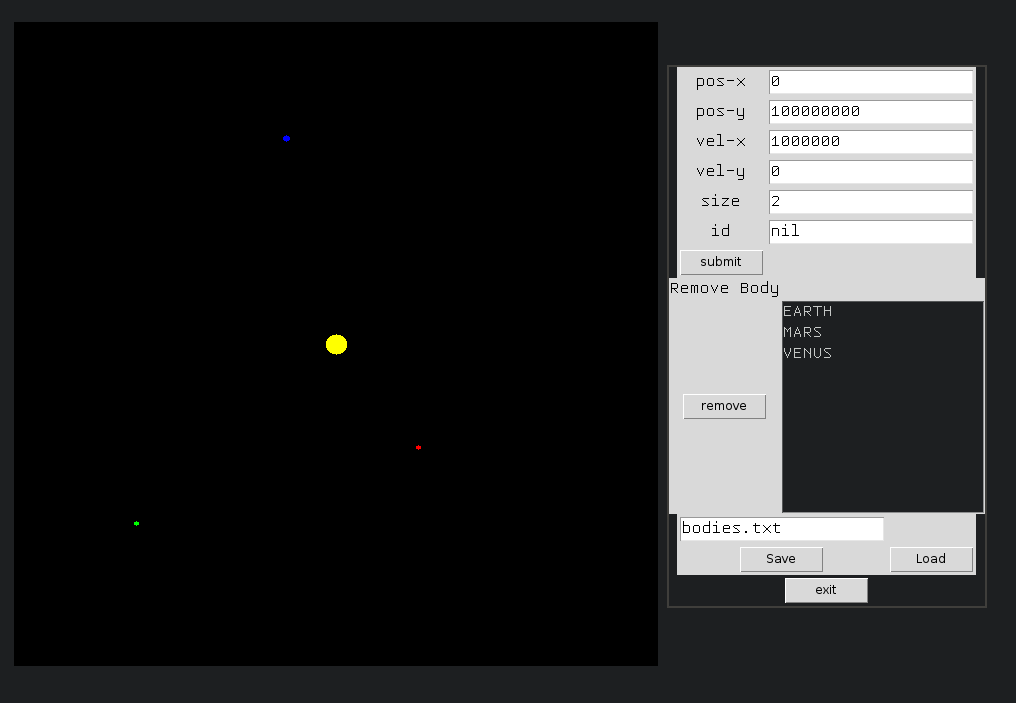
\includegraphics[width=\textwidth]{./img/start.png}
\end{figure}

\section{Running the simulation}
\subsection{Typical}
\paragraph{Expected Outcome}
The planets will orbit the sun on their respective paths, the patterns should be
repetitive and should not change.
\paragraph{Actual Outcome}
The planets all move along their expected paths, with no problems.

\subsection{Extreme}
\paragraph{Expected Outcome}
The planets will orbit the sun on their respective paths, the patterns should be
repetitive and should not change.
\paragraph{Actual Outcome}
The simulation continues to run despite having a lot more bodies than should be
needed, some of which were off the screen.
\begin{figure}[H]
	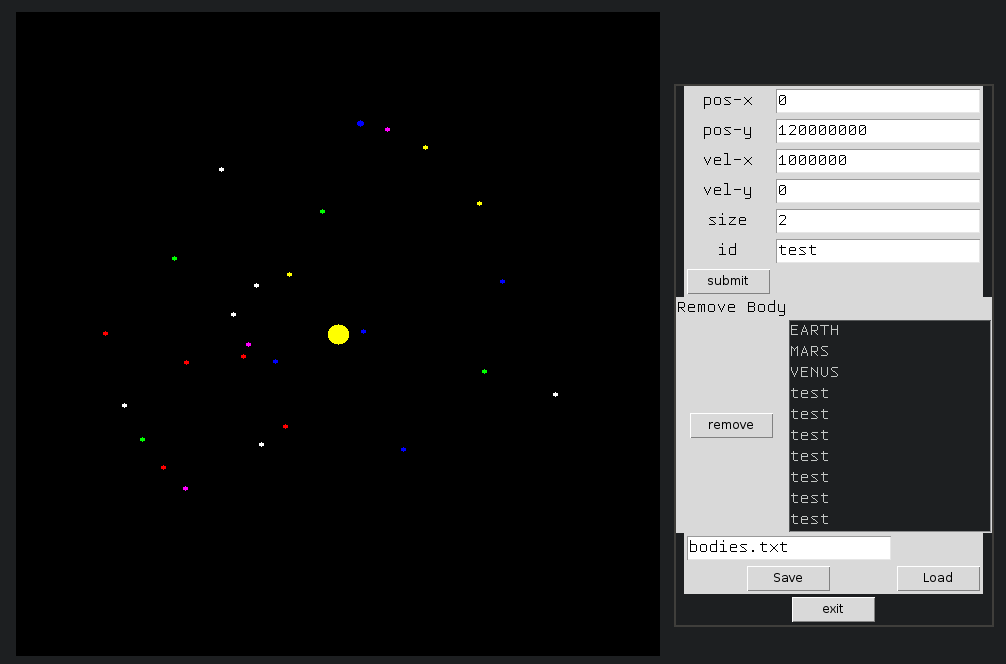
\includegraphics[width=\textwidth]{./img/run.png}
\end{figure}


\section{Adding a body}
\subsection{Typical}
\paragraph{Expected Outcome}
The body will be added to the simulation and it will follow its path, which
depends on the parameters it was added with.
\paragraph{Actual Outcome}
The body is added with the given parameters, and follows the path of its orbit.
\begin{figure}[H]
	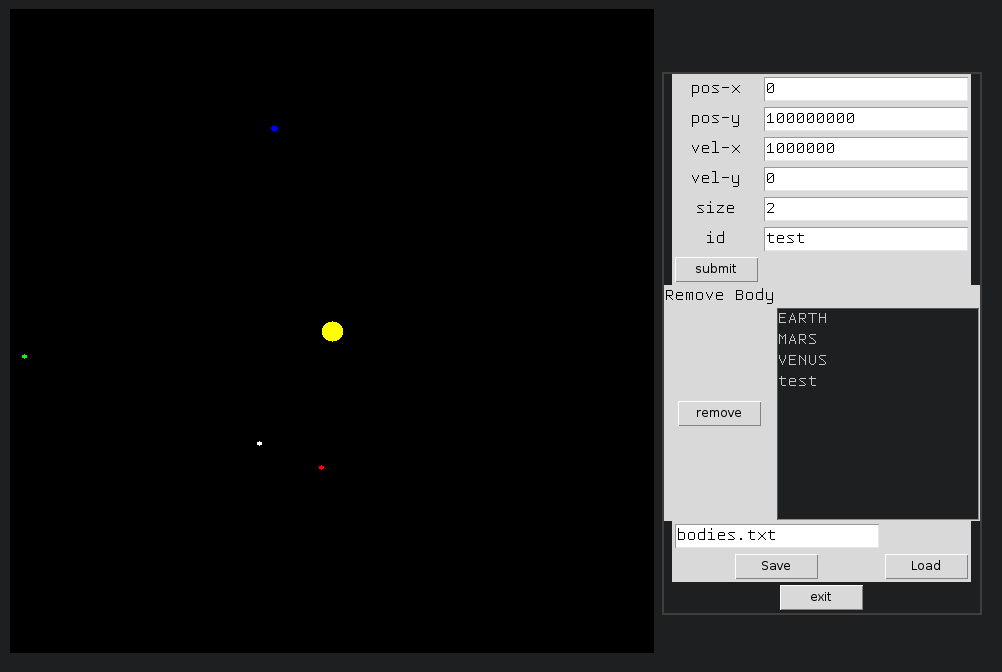
\includegraphics[width=\textwidth]{./img/add1.png}
\end{figure}

\subsection{Erroneous}
\paragraph{Expected Outcome}
A message box will appear to tell the user that the parameters given are not
valid, and should be changed.
\paragraph{Actual Outcome}
A message box appears warning the user, however the system still adds the body
with the erroneous value, causing the program to crash.
\begin{figure}[H]
	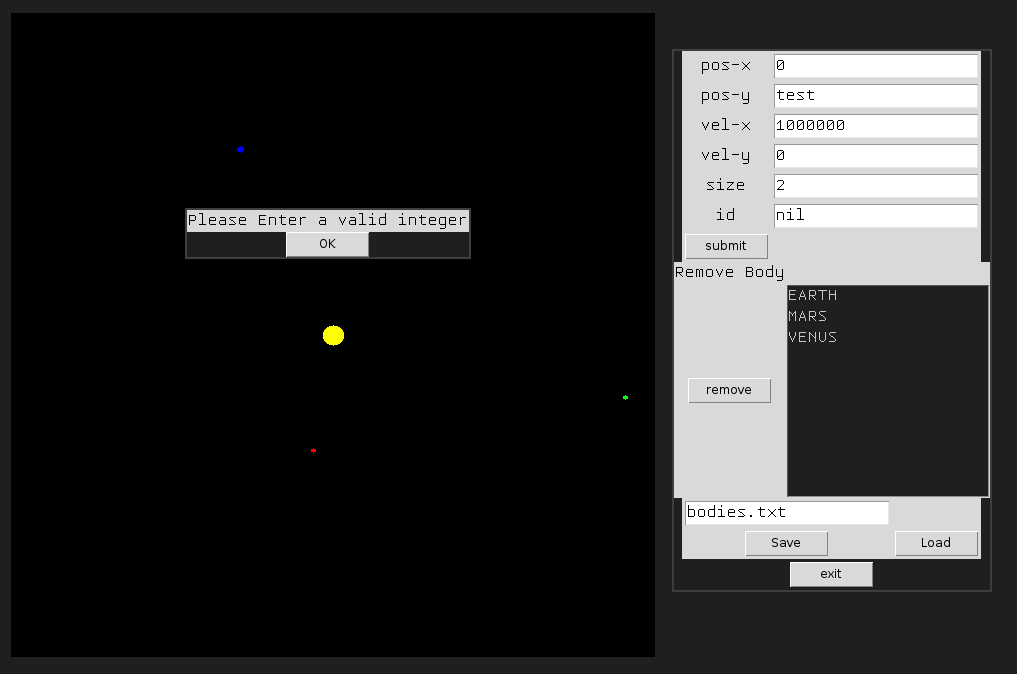
\includegraphics[width=\textwidth]{./img/add2.png}
\end{figure}
\paragraph{Comments and Corrective actions}
The code before initially was this lambda function that is called when the
submit button is pressed. 
\begin{lstlisting}
	(lambda ()
	   (apply #`add-body
		  (append
		   (mapcar #`parse-int
			   (list
			    (ltk:text in-posx)
			    (ltk:text in-posy)
			    (ltk:text in-velx)
			    (ltk:text in-vely)))
		   (list :size (parse-int (ltk:text in-size))
			 :id (ltk:text in-id)
			 :colour `a)))
	   (listbox-update bod-list))
\end{lstlisting}
And parse-int looked like this:
\begin{lstlisting}
(defun parse-int (str)
  "Converts a string to an int, and creates an error message if its invalid"
  (let ((int (parse-integer str :junk-allowed 't)))
    (if int
	int
	(error-message "Please Enter a valid integer"))))
\end{lstlisting}
As you can see, it does check if parse-integer return a valid answer, but the
only error handling it did was to create a message for the user.
\subsection{Extreme}
\paragraph{Expected Outcome}
A message box will appear to tell the user that the values given could cause
problems with the simulation, and it is advised that they change them.
\paragraph{Actual Outcome}
\paragraph{Comments and Corrective actions}


\section{Removing a body}
\subsection{Typical}
\paragraph{Expected Outcome}
The selected body will be removed from the simulation.
\paragraph{Actual Outcome}
\paragraph{Comments and Corrective actions}

\subsection{Erroneous}
\paragraph{Expected Outcome}
A message box will appear to tell the user that they need to select a body
before they can remove one.
\paragraph{Actual Outcome}
\paragraph{Comments and Corrective actions}


\section{Saving the system to a file}
\subsection{Typical}
\paragraph{Expected Outcome}
The current details of the simulation will be saved to a file, with the name
given by the user.
\paragraph{Actual Outcome}
\paragraph{Comments and Corrective actions}

\subsection{Erroneous}
\paragraph{Expected Outcome}
A message box will appear to tell the user that the file name they have entered
is not valid, and should be changed before saving.
\paragraph{Actual Outcome}
\paragraph{Comments and Corrective actions}

\subsection{Extreme}
\paragraph{Expected Outcome}
The current details of the simulation will be saved to a file, with the name
given by the user.
\paragraph{Actual Outcome}
\paragraph{Comments and Corrective actions}


\section{Loading the system from a file}
\subsection{Typical}
\paragraph{Expected Outcome}
The details of the saved simulation will be loaded from the given file and will
replace the current system.
\paragraph{Actual Outcome}
\paragraph{Comments and Corrective actions}

\subsection{Erroneous}
\paragraph{Expected Outcome}
A message box will appear to tell the user that the file name they have entered
is invalid, or does not exist, and that they should enter a new one.
\paragraph{Actual Outcome}
\paragraph{Comments and Corrective actions}

\subsection{Extreme}
\paragraph{Expected Outcome}
The details of the saved simulation will be loaded from the given file and will
replace the current system.
\paragraph{Actual Outcome}
\paragraph{Comments and Corrective actions}


